\documentclass[10pt]{article}

% Lines beginning with the percent sign are comments
% This file has been commented to help you understand more about LaTeX

% DO NOT EDIT THE LINES BETWEEN THE TWO LONG HORIZONTAL LINES

%---------------------------------------------------------------------------------------------------------

% Packages add extra functionality.
\usepackage{
	times,
	graphicx,
	epstopdf,
	fancyhdr,
	amsfonts,
	amsthm,
	amsmath,
	algorithm,
	algorithmic,
	xspace,
	hyperref}
\usepackage[left=1in,top=1in,right=1in,bottom=1in]{geometry}
\usepackage{sect sty}	%For centering section headings
\usepackage{enumerate}	%Allows more labeling options for enumerate environments
\usepackage{epsfig}
\usepackage[space]{grffile}
\usepackage{booktabs}
\usepackage{amsmath}
\usepackage[super]{nth}
\usepackage{array}

% This will set LaTeX to look for figures in the same directory as the .tex file
\graphicspath{.} % The dot means current directory.

\pagestyle{fancy}

\lhead{\YOURID}
\chead{\MyLang: Language Specification}
\rhead{\today}
\lfoot{CSCI 334: Principles of Programming Languages}
\cfoot{\thepage}
\rfoot{Spring 2022}

% Some commands for changing header and footer format
\renewcommand{\headrulewidth}{0.4pt}
\renewcommand{\headwidth}{\textwidth}
\renewcommand{\footrulewidth}{0.4pt}

% These let you use common environments
\newtheorem{claim}{Claim}
\newtheorem{definition}{Definition}
\newtheorem{theorem}{Theorem}
\newtheorem{lemma}{Lemma}
\newtheorem{observation}{Observation}
\newtheorem{question}{Question}

\setlength{\parindent}{0cm}
%---------------------------------------------------------------------------------------------------------

% DON'T CHANGE ANYTHING ABOVE HERE

% Edit below as instructed
\newcommand{\MyLang}{GeoDraw}	% Replace MyLang with your language name #
\newcommand{\PartnerOne}{Isabel Grondin}	% Replace PartnerOne with your name #
\newcommand{\PartnerTwo}{Meredith Wolf}	% Replace PartnerTwo with your partner's name #
\newcommand{\YOURID}{\PartnerOne{} + \PartnerTwo{}} % Remove \PartnerTwo if working alone.


\title{\MyLang: Language Specification}
\date{Spring 2022}
\author{\PartnerOne{} and \PartnerTwo{}} % Remove \PartnerTwo if working alone.

\begin{document}
\maketitle

\vspace{\baselineskip}	% Add some vertical space

% Refer to the lab handouts to determine what should go in each of these sections.  Each lab is additive.  So lab 8 should include everything you wrote in lab 7.  Lab 9 should include everything you wrote in lab 8, etc.

\section{Introduction}

GeoDraw is a language that lets you use basic math equations (lines, circles, parabolas, etc) to construct basic cartoon drawings. Shading can be done by using inequalities. This is inspired by a project in high school that was designed to help us learn more about geometry. It was difficult to find a graphing calculator online that made this particular project easy. GeoDraw will be a be a fun educational tool to strengthen students knowledge of geometrical equations.
\\\\This language can also be viewed as a gentle introduction to computer graphics, which use much more complex mathematical equations, and to programming more generally. For that reason simplicity is an important part of our language design.


\section{Design Principles}

Our guiding principles are simplicity and readability. Since this language is targeted towards younger populations, who are most likely being introduced to programming, we want the language to be fairly intuitive. Furthermore, GeoDraw is a tool aiding students in learning graphing skills, and we do not want the complexity of the language to detract from that core objective.

\section{Example Programs}

\textbf{Example 1:}

\begin{verbatim}
canvas(5,5)
draw(y = 1, col=‘#000000’, brushType =‘simple’);
\end{verbatim}

\begin{center}
		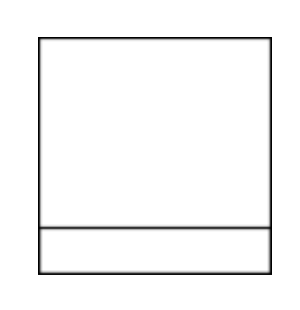
\includegraphics[scale=0.8]{images/exampleProgram1}
\end{center}

\textbf{Example 2:}

\begin{verbatim}
canvas(10, 10)
draw(y = x, bounds=(2<x<8), col=‘#ff0000’, brushType =‘simple’)
\end{verbatim}

\begin{center}
		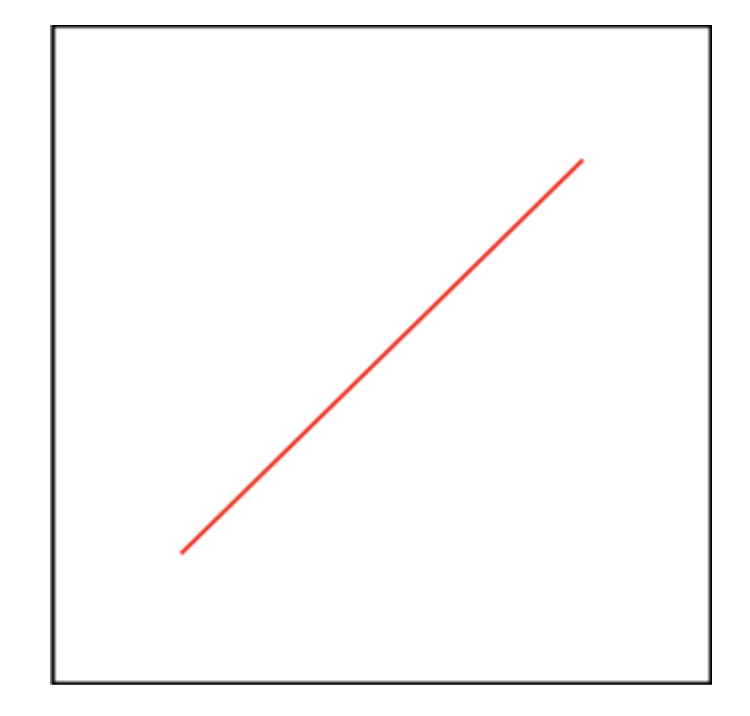
\includegraphics[scale=0.5]{images/exampleProgram2}
\end{center}

\textbf{Example 3:}

\begin{verbatim}
canvas(8, 8)
draw(y = abs(x-4), col=‘#0000ff’, brushType=‘simple’)
\end{verbatim}

\begin{center}
		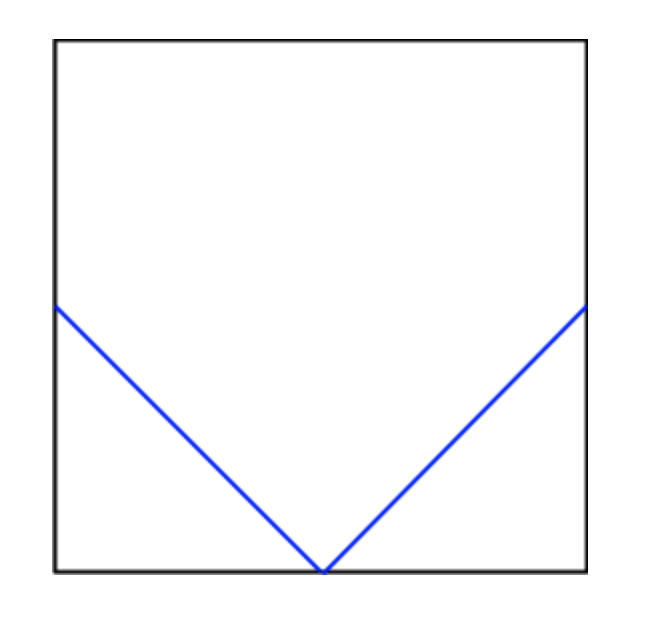
\includegraphics[scale=0.5]{images/exampleProgram3}
\end{center}


\section{Language Concepts}
The core concept a user needs to understand for GeoDraw, is how to create an equation of the form $<Y><eq><Exp>$ to generate the desired line and shading effect. An Expression,$<Exp>$ consists of the primitive data types $X$, real numbers and operations. Draw is a combining form in our language that is made up of an equation, color, bounds, and brush style.


\section{Syntax}

\textbf{Primitives:}

\begin{itemize}
\item x,y
\item real numbers
\item colors (hex codes)
\item operations(+ - / * sin cos pow sqrt abs)
\item equalities ($< > =$)
\end{itemize}

\newpage
\textbf{Combining Forms:}
	\begin{itemize}
	\item Math expressions
			\begin{itemize}
			\item x
			\item Real numbers
			\item Mult of Expr * Expr
			\item Sub of Expr * Expr
			\item Div of Expr * Expr
			\item Add of Expr * Expr
			\item Sin of Expr
			\item Cos of Expr
			\item Sqrt of Expr
			\item Abs of Expr
			\item Pow of Expr * Expr
			\end{itemize}
	\item Equations
			\begin{itemize}
			\item $<y> <Eq> <Expr>$
			\end{itemize}
	\item Bounds (default: canvas boundaries)
			\begin{itemize}
			\item \textbf{R} $< y <$ \textbf{R}
			\item \textbf{R} $< x <$ \textbf{R}
			\end{itemize}
	\item Canvas → takes height and width
	\item Point → real number * real number
	\item Brush Style → List of points in 5 x 5 square
	\begin{itemize}
	\item Real numbers must be between 0 and 5
	\end{itemize}
	\item Drawing → Equation * Bounds * Color * Brush Style

\end{itemize}


\section{Semantics}

\begin{enumerate}[i]
	\item We are going to use the following primitive types in generating an expression: x, y, real numbers, operations and equality symbols. These will allow the users to generate the line of almost any equation they wish to draw. Color will also be a primitive type that can be used for shading and drawing lines with different colors.
	\item First, the user must create a canvas by inputting a height and width. Drawings will end at x and y unless other limits are specified. Drawings are the main elements in the language. They are a combination of an equation, its bounds, a color, and a brush style. Equations must have the y variable on the left, an $=, <,$ or $>$, followed by a mathematical expression. Bounds denote the limits of the equation for x, y, or both. Mathematical expressions combine our operations, real numbers, and the x variable. Brush styles consist of a list of points, which we will connect to look like brush strokes.
	\item \textbf{Hierarchy Drawing:}\\
	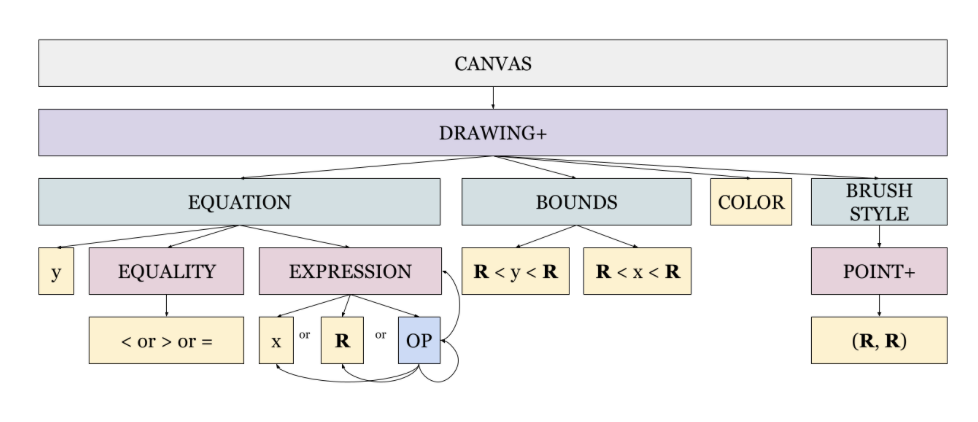
\includegraphics[scale=0.7]{images/hierarchyDrawing} \\
	\item \textbf{AST for Example 1:}\\
	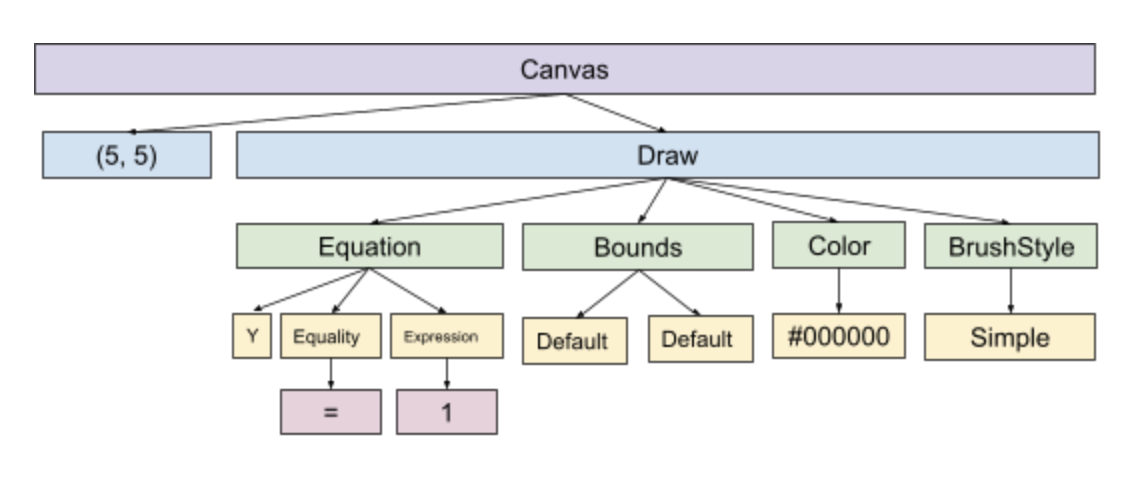
\includegraphics[scale=0.7]{images/ASTExample1}

	\textbf{AST for Example 2:} \\
	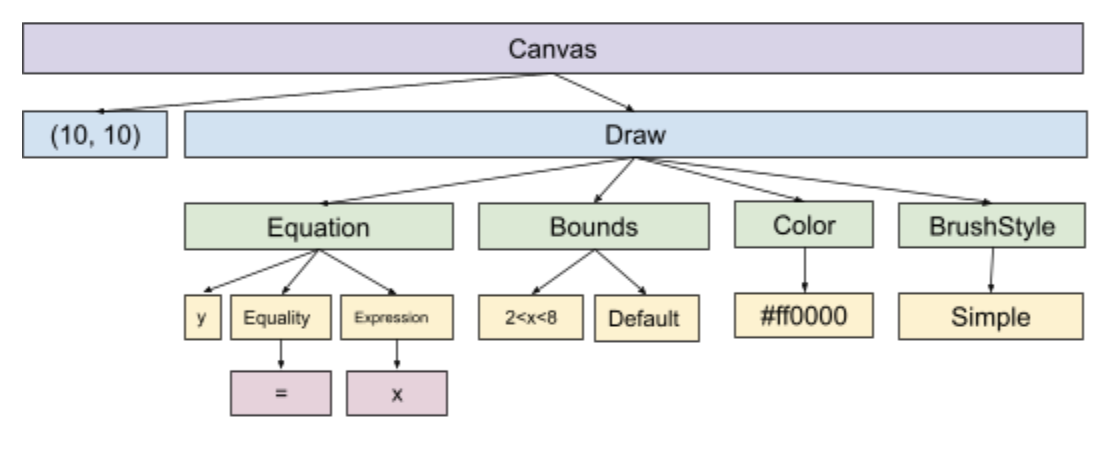
\includegraphics[scale=0.7]{images/ASTExample2}

	\textbf{AST for Example 3:}\\
	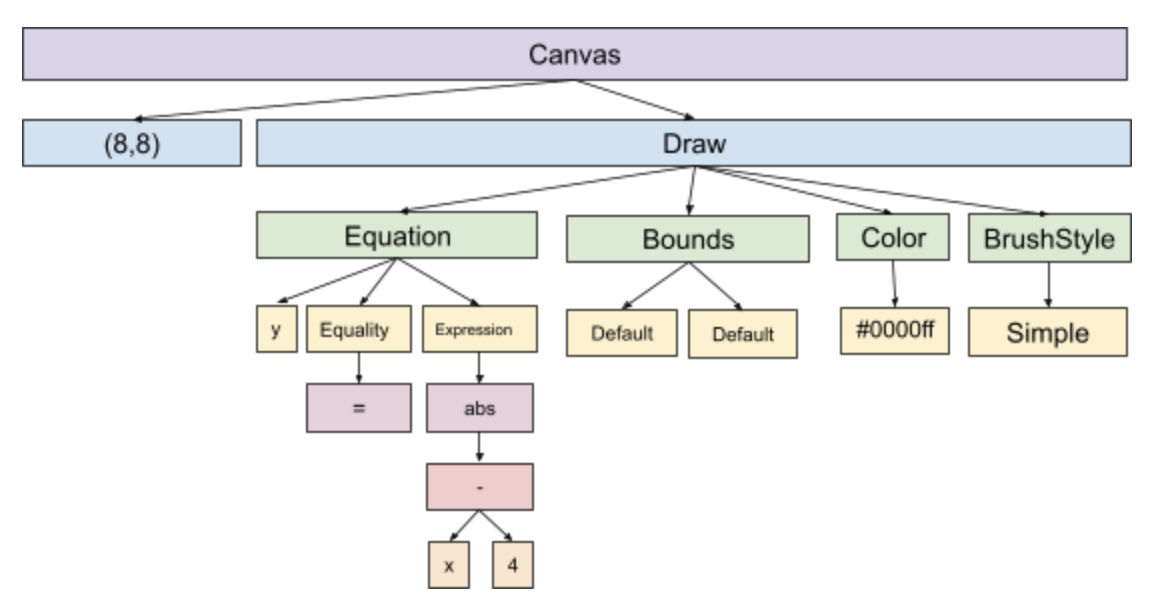
\includegraphics[scale=0.7]{images/ASTExample3}

	\item No, our programs do not read any input. However, the user can input a program as a file so they do not have to retype all the commands.
	\item The output of evaluating the program is a drawing consisting of the lines specified in the program. This will be in the form of an SVG file.
	\item First, we get the canvas size. \\
	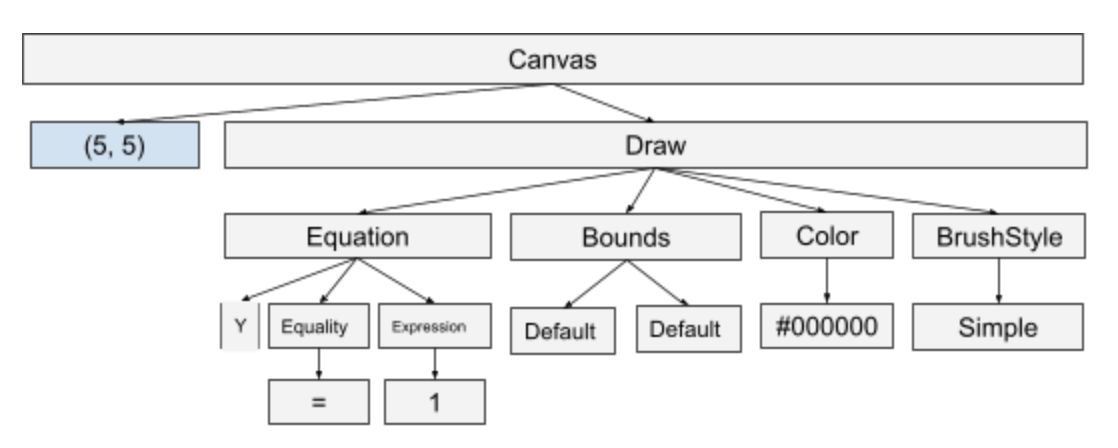
\includegraphics[scale=0.7]{images/seq1} \\
	Then, we get the equation that we want to draw. \\
	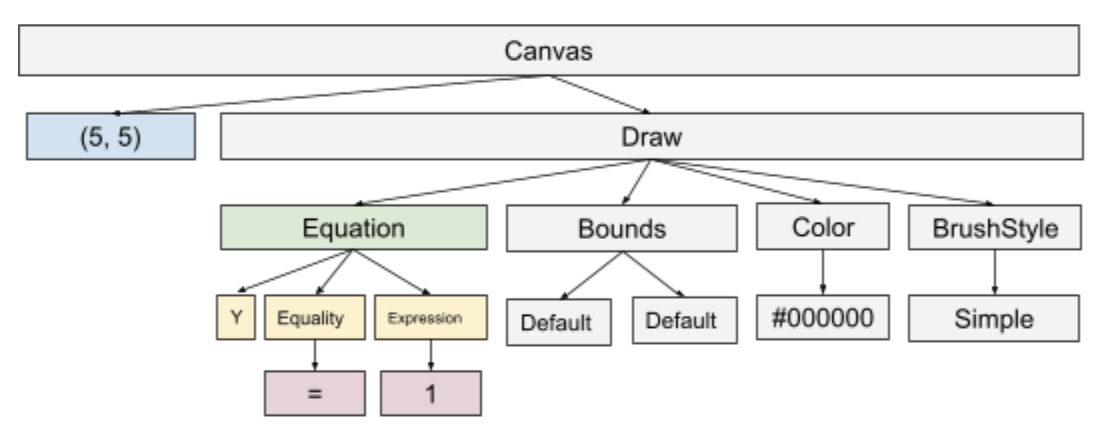
\includegraphics[scale=0.7]{images/seq2} \\
	\newpage
	Next, we get the bounds for where to evaluate $x$ and $y$. If they are default, they are the canvas size. So in this case, $0 <= x <= 5$ and $0 <= y <= 5$. \\
	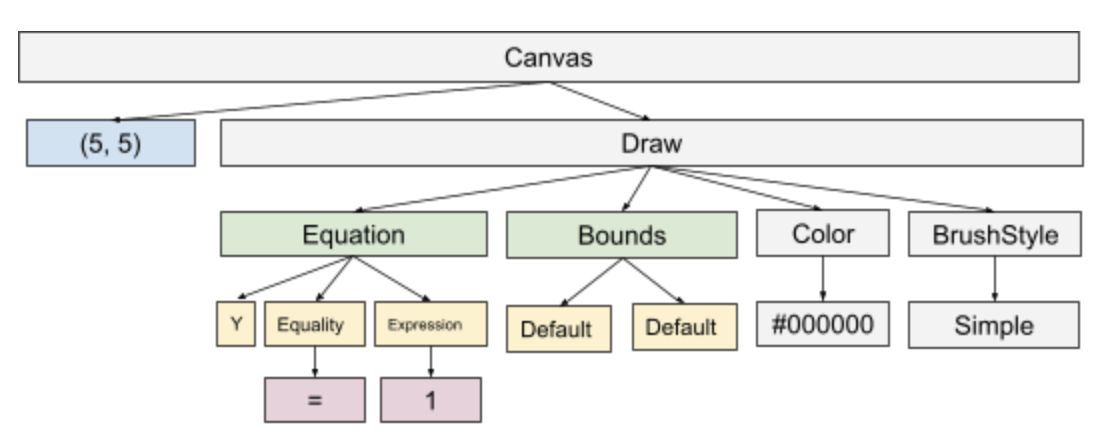
\includegraphics[scale=0.7]{images/seq3} \\
	Then, we get the hex code for the color we would like to draw with. In this case it is \#000000 for black. \\
	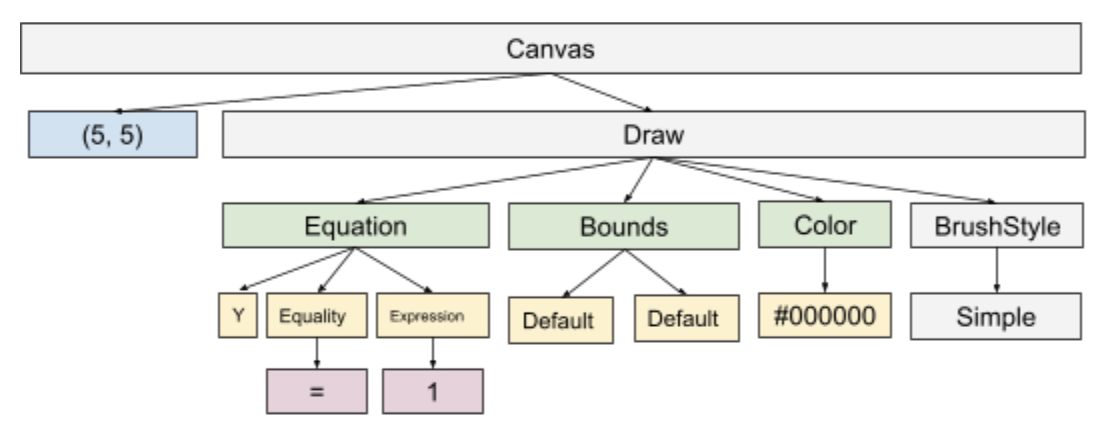
\includegraphics[scale=0.7]{images/seq4} \\
	Then we get the brushStyle. In this case, it is ‘simple’ for just a single line.\\
	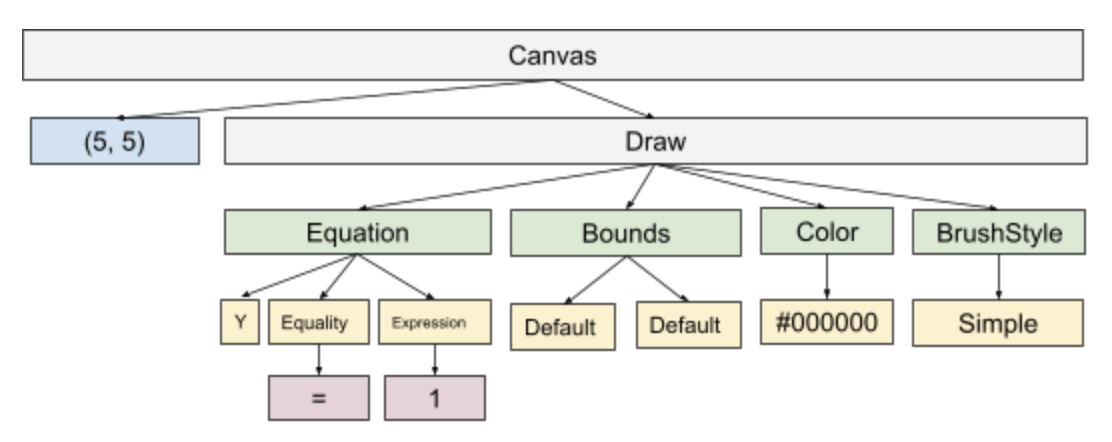
\includegraphics[scale=0.7]{images/seq5} \\
	\newpage
	Now, we have everything we need to draw the equation, so we do that using SVG.\\
	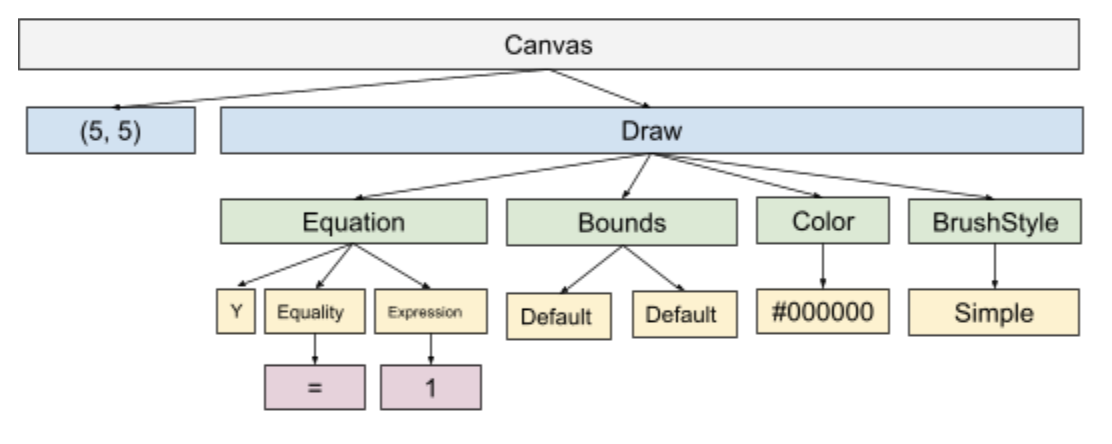
\includegraphics[scale=0.7]{images/seq6} \\
	We have no more draw commands left to evaluate, so we are done. \\
 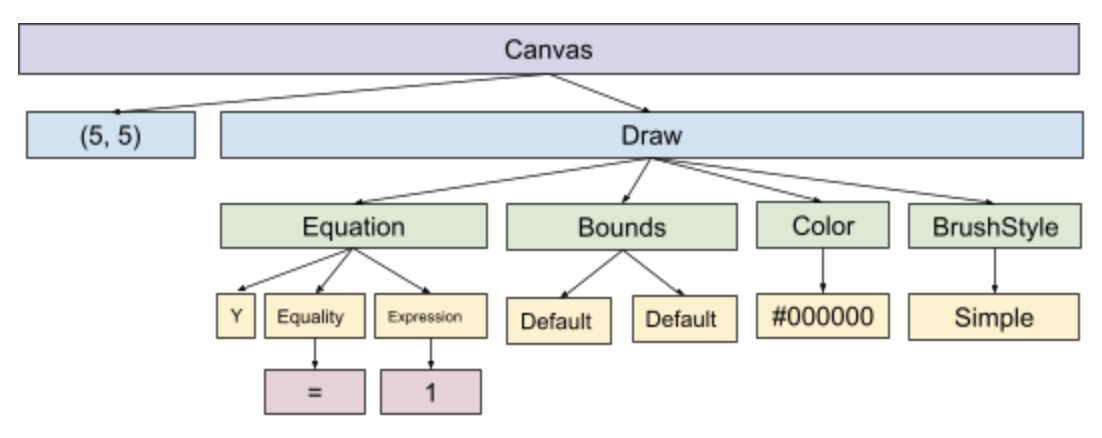
\includegraphics[scale=0.7]{images/seq7} \\

\end{enumerate}


% DO NOT DELETE ANYTHING BELOW THIS LINE
\end{document}
